
\documentclass[12pt,a4]{article}


\newcommand{\handoutdate}{2020-03-05}
\newcommand{\firstduedate}{2020-03-10}
\newcommand{\finalduedate}{2020-03-17 before class}




\usepackage{graphicx,amsmath,amssymb,amsthm, boxedminipage}



\usepackage{algorithm}
\usepackage{algpseudocode}


\newtheorem{theorem}{Theorem}%[section]
\newtheorem{proposition}[theorem]{Proposition}
\newtheorem{lemma}[theorem]{Lemma}
\newtheorem{corollary}[theorem]{Corollary}
\newtheorem{definition}[theorem]{Definition}



\newcommand{\scalar}[2]{\ensuremath{\langle #1, #2\rangle}}
\newcommand{\floor}[1]{\left\lfloor #1 \right\rfloor}
\newcommand{\ceil}[1]{\left\lceil #1 \right\rceil}
\newcommand{\norm}[1]{\|#1\|}
\newcommand{\pfrac}[2]{\left(\frac{#1}{#2}\right)}
\newcommand{\nth}[1]{#1\textsuperscript{th}}

% \newcommand{\nth}[1]{#1\textsuperscript{th}}
\newcommand{\E}{\mathop{\mathbb{E\/}}}
\newcommand{\N}{\mathbb{N}}

\newcommand{\R}{\mathbb{R}}

\newtheorem{exercise}[theorem]{Exercise}
\newtheorem{exerciseD}[theorem]{*Exercise}
\newtheorem{exerciseDD}[theorem]{**Exercise}

\let\oldexercise\exercise
\renewcommand{\exercise}{\oldexercise\normalfont}

\let\oldexerciseD\exerciseD
\renewcommand{\exerciseD}{\oldexerciseD\normalfont}

\let\oldexerciseDD\exerciseDD
\renewcommand{\exerciseDD}{\oldexerciseDD\normalfont}


 
\begin{document}

\date{}

\title{CS 217 -- Algorithm Design and Analysis \\ 
  \vspace{3mm}
{\large	Shanghai Jiaotong University, Fall 2019\\
}
}
\maketitle

\noindent
Handed out on \handoutdate{}\\
First submission and questions due on \firstduedate{}\\
You will receive feedback from the TA.\\
Final submission due on \finalduedate{}


\section{Bit Complexity, Recursion, and Dynamic Programming}

\subsection{Bit Complexity of Euclid's Algorithm}

We have proved that Euclid's algorithm for computing $\gcd(a,b)$ makes at most
$O(\log a)$ iterations. What is the overall running time? Each iteration computes
$u \mod v$ for some integers. This can be done by integer division. What is its running time?
There are very sophisticated algorithms, but python probably does not come with them. 
Recall the ``school method'' for dividing integers. Have a look at the pdf slides on the 
webpage for an illustration of the school method. It is especially simple if we are dealing
with binary numbers. If $a$ and $b$ have at most $n$ bits, then the school method 
has complexity $O(n^2)$.
\begin{exercise}
  Show the following, more precise bound of the school method for integer division:
  If $a$ has $n$ bits and $b$ has $k$ bits, then the school method can be implemented
  to run in $O( k(n-k))$ operations.
\end{exercise}
\begin{proof}
		
\end{proof}
\begin{exercise}
  Show that the bit complexity of Euclid's algorithm, using the school method
  to compute $a \mod b$, is $O(n^2)$. That is,
  if $a$ and $b$ have at most $n$ bits, then $\gcd(a,b)$ makes $O(n^2)$ bit operations.\\
  
  In order to do so, here is python code of the Euclidean algorithm:
\begin{verbatim}
  def euclid(a,b):
    while (b > 0):
        r = a % b # so a = bu+r
        if (r == 0):
            return b
        s = b % r # so b = rv + s
        a = r
        b = s
    return a
\end{verbatim}
Don't be afraid to introduce notation! I recommend to let $n$ denote the number of bits of $a$.
Take some other letters for the number of bits in $b$ and so on.
\end{exercise}
\begin{proof}
		Assume that $\gcd\left( a,b \right) $ takes $t$ iterations and $t \le  2n$. To better represent our ideas.  Let's introduce
		some notations. Conside a process of iterations as follows:
		\[
				\gcd\left( a,b \right) = \gcd\left( x_{t},x_{t-1} \right) \to 
				\gcd\left( x_{t-1},x_{t-2} \right) \to \ldots \to \gcd\left( x_1,0 \right) 
		.\] 
		And $\forall 1\le k\le t$ let $x_{k}$ has $y_{k}$ bits. We know $y_{t}\le n$ plus $x_{k}>x_{k-1}$.
		Hence $\forall k, y_{k}\ge y_{k-1}$.

		Let the operations of all iterations be $T$. And the operations of  $k$th iteration be $T_{k}$. 
		Now apply the conclusion of Exercise 1, we have
		\begin{align*}
				T &= \sum_{k=1}^{t} T_{k} \\
				  &\le \lambda \sum_{k=1}^{t} y_{k}\left( y_{k}-y_{k-1} \right) \\ 
				& \le \frac{\lambda}{2}\left( \sum_{k=1}^{t} \left( y_{k}-y_{k-1} \right)^2 + y_t^2 \right) \\
				  & \le  \frac{\lambda}{2} \left( \sum_{k=1}^{t} \left( y_{k}-y_{k-1} \right)  \right)^2+ \frac{\lambda}{2} y_{t}^2\\
				  & \le  \frac{\lambda}{2} n^2
		.\end{align*} 
		Hence $\gcd\left( a,b \right) $ makes $O\left( n^2 \right) $ operations.
\end{proof}
\subsection{Computing the Binomial Coefficient}

Next, we will investigate the binomial coefficient ${n \choose k}$, which 
you might also know by the notation $C^k_n$. The number ${n \choose k}$ is defined
as the number of subsets of $\{1,\dots,n\}$ which have size exactly $k$. 
This immediately shows that ${n \choose k}$ is $0$ if $k$ is negative or larger than $n$.
You might have seen the following recurrence:
\begin{align*}
 {n \choose k} & = {n-1 \choose k-1} + {n-1 \choose k} \textnormal{ if } n,k \geq 0 \ .
\end{align*}

\begin{exercise}[A Recursive Algorithm for the Binomial Coefficient]
  Using pseudocode, write a recursive algorithm computing
  ${n \choose k}$. Implement it in python! What is 
  the running time of your algorithm, in terms of $n$ and $k$? Would you say it is an efficient
  algorithm? Why or why not?
\end{exercise}
\begin{proof}
		\begin{algorithm}[b]
				\caption{A function $f$ using recursive algorithm.}
				\KwIn{input parameters $n,k$}
				\KwOut{$ {n\choose k }$}
				\LinesNumbered
				\If{$n=k$ or $k=0$} {
						return $1$
				} 
				\Else {
						return $f\left( n-1,k-1 \right) + f\left( n-1,k \right) $
				}
		\end{algorithm}
		The python implementation
\begin{verbatim}
  def f(n,k):
    if n < k:
        return 0
    elif n == k or k == 0:
        return 1
    else:
        return f(n-1,k-1)+f(n-1,k)
\end{verbatim}
		It's not a good algorithm.
\end{proof}
\begin{exercise}[A Dynamic Programming Algorithm for the Binomial Coefficient]
  Using pseudocode, write a dynamic programming algorithm
  computing ${n \choose k}$. Implement it in python! What is it running time
  in terms of $n$ and $k$?
  Would you say your algorithm is efficient? Why or why not?
\end{exercise}
\begin{proof}
		\begin{algorithm}[h]
				\caption{A function $g$ using dynamic algorithm.}
				\KwIn{input parameters $n,k$}
				\KwOut{$ {n\choose k }$}
				\LinesNumbered
				\If{$n=k$ or $k=0$} {
						return $1$
				} 
				\Else {
						return $f\left( n-1,k-1 \right) + f\left( n-1,k \right) $
				}
				
		\end{algorithm}
\end{proof}

\begin{exercise}[Binomial Coefficient modulo 2]
  Suppose we are only interested in whether ${n \choose k}$ is even or odd,
  i.e., we want to compute ${n \choose k}  \mod 2$. You could do this by computing 
  ${n \choose k}$ using dynamic programming and then taking
  the result modulo $2$. What is the running time? Would you say this algorithm
  is efficient? Why or why not?
\end{exercise}
\begin{proof}
	Here is another method. Following is implement in python.
\begin{verbatim}
  def C(n, k):
    if n & k == k:
        return 1;
    else:
        return 0;
\end{verbatim}

Now, let's proof this simple algorithm why it's correct.
According to \textbf{Lucas Theorem}.
\begin{theorem}
	\textbf{(Lucas Theorem)} For non-negative integers \textit{m} and \textit{n} and a prime \textit{p}, the following congruence relation holds:
	$${m \choose n} \equiv \prod_{i=0}^k {m_i \choose n_i} ( mod\ p),$$
	where
	$$m=m_kp^k+m_{k-1}p^{k-1}+\cdots+m_1p+m_0$$,
	and
	$$n=n_kp^k+n_{k-1}p^{k-1}+\cdots+n_1p+n_0$$
	are the base p expansions of m and n respectively. This uses the convention that ${m\choose n}=0$ if $m<n$.
\end{theorem}
Here, we let p = 2, and we have ${0 \choose 0}={1\choose 0}={1 \choose 1}=1$ and ${0 \choose 1}=0$. Hence, we get ${n\choose k}\equiv 1 (mod\ 2)$ if and only if every bit of k is less than that of n in binary representation. That means $n\ and\ k = k$.
The time complexity of this algorithm is $\Theta(log(n))$

\end{proof}
\begin{exercise}
  Remember the ``period'' algorithm for computing $F'_n := (F_n \mod k)$ discussed in class:
  (1) find some $i,j$ between $0$ and $k^2$ for which 
  $F'_{i} =  F'_{j}$ and $F'_{i+1} = F'_{j+1} $. 
  Then for $d := j-i$ the sequence $F'_{n}$ will repeat every $d$ steps, as there will be a cycle.
  This cycle can either be a ``true cycle'' or a ``lasso'':
  \begin{center}
  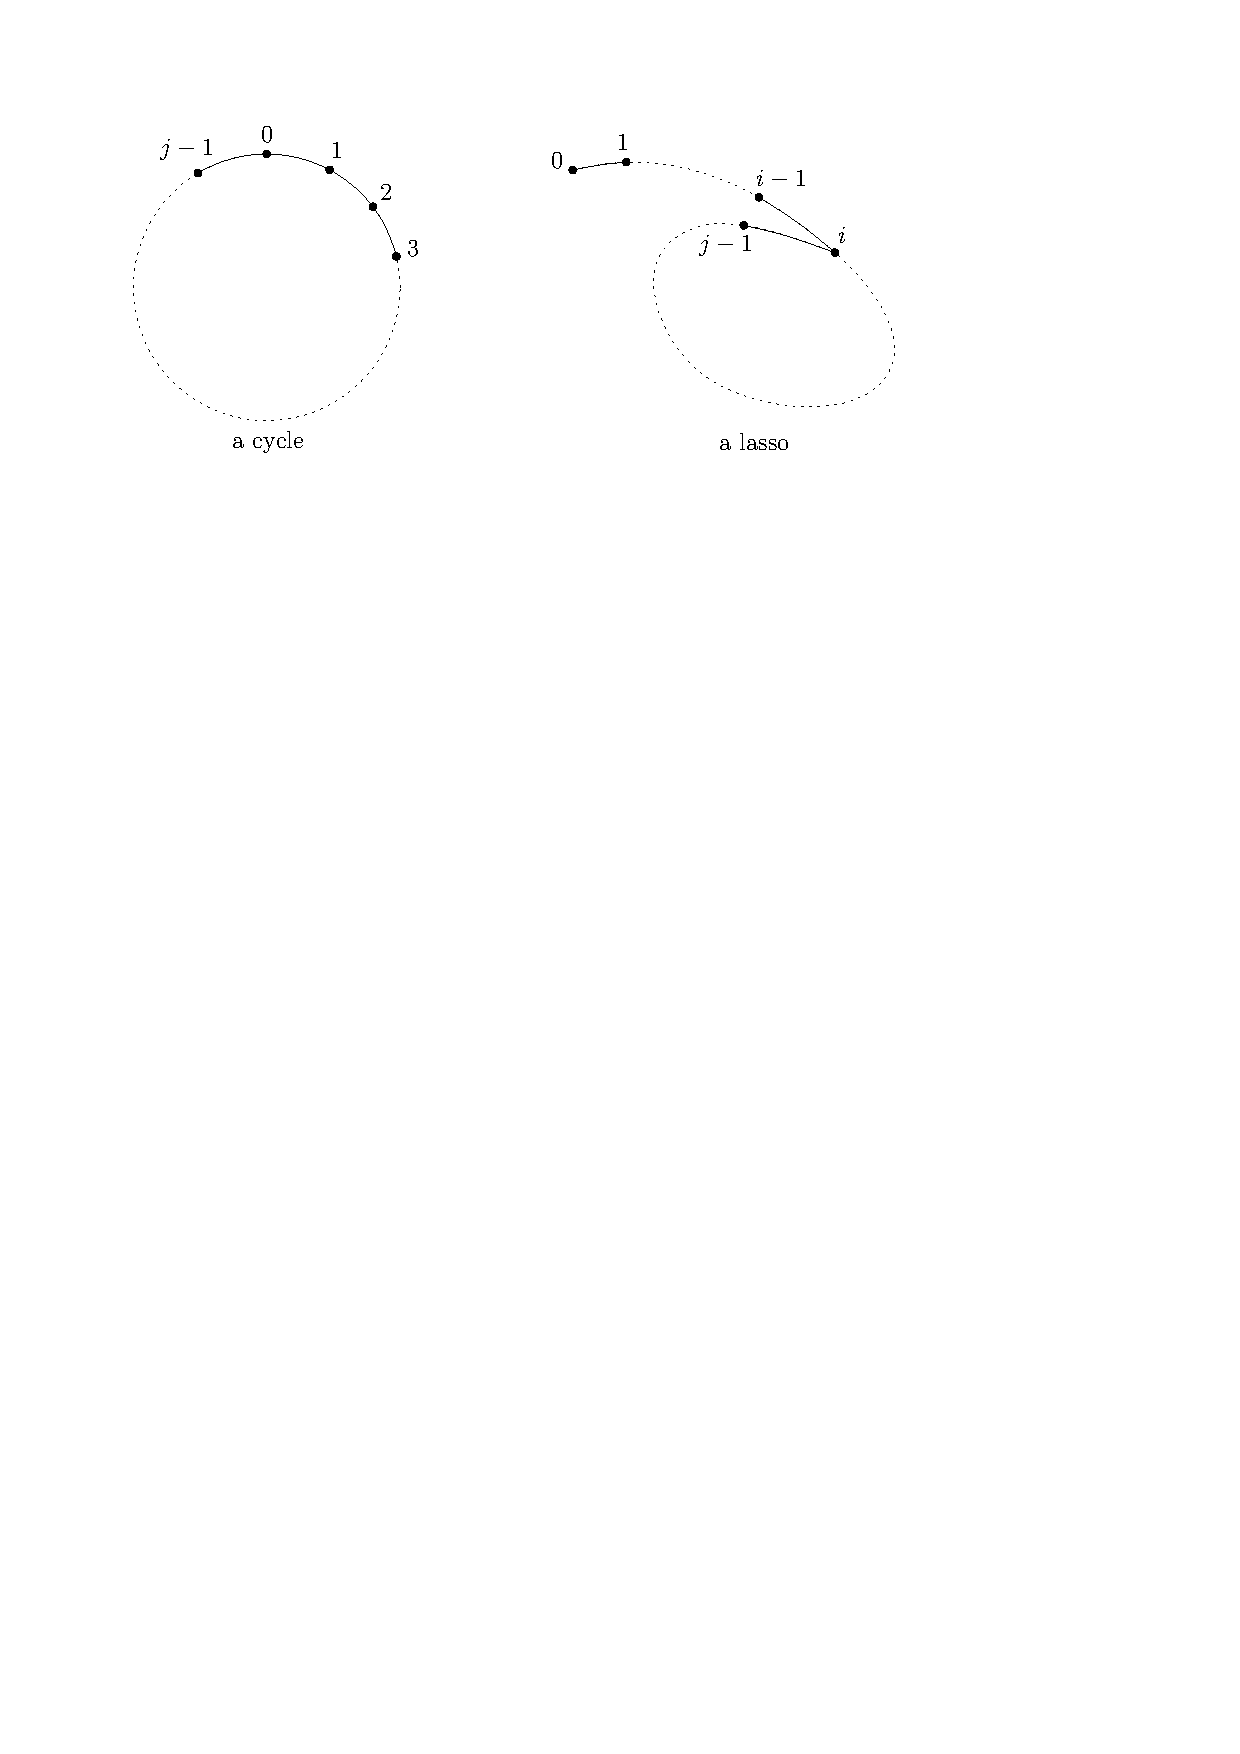
\includegraphics[width=0.8\textwidth]{../figures/cycle-and-lasso.pdf}
  \end{center}
  
  Show that a lasso cannot happen. That is, show 
  that the smallest $i$ for which this happens is $0$, i.e, for some $j$ we have
  $F'_0 = F'_j$ and $F'_1 = F'_{j+1}$ and thus $F'_n = F'_{n \textnormal{ mod }  j}$.
\end{exercise}
  
\begin{proof}
		Consider a pair $g\left( i \right) =\left( F'_{i-1},F'_{i} \right) , i\ge 0$. We know that
		$\forall i, g\left( i \right) \in [0,n)\times [0,n)$ which is a finite set with $k^2$ members.

		Consider the following set 
		\[
				A = \{ g\left( 1 \right) ,g\left( 2 \right) ,\ldots, g\left( k^2 \right) , g\left( k^2+1 \right) \} 
		.\] 
		By \textbf{Pigeonhole Principle}, we know that $\exists r< s\in \{1,2,\ldots,k^2+1\} $ such that 
		$g\left( r \right) =g\left( s \right) $ which is
		\[
				F'\left( r-1 \right) = F'\left( s-1 \right) , \quad F'\left( r \right)  = F'\left( s \right) 
		.\] 
		Since $F'\left( r-2 \right)$ is determined by $F'\left( r \right) -F'\left( r-1 \right) $, we can imply that 
		\[
				F'\left( 0 \right)  = F'\left( s-r \right) , \quad F'\left( 1 \right)  = F'\left( s-r+1 \right) 
		.\] 
		Hence this cycle is a ``true cycle".
\end{proof}



\paragraph{Python.} Please write your code in python. It is a very simple programming
language. If you do not know any python, I can put same example code online and 
you can learn by example. Also, for this homework you definitely need a Big Integer class
since numbers with ten thousand digits do not fit into any \texttt{long long int} or similar.
Python automatically supports Big Integer, so there is no problem here.


\end{document}
